\documentclass[a4paper, 14pt]{article}


\usepackage{hyperref}
\usepackage{upgreek}
\usepackage[usenames,dvipsnames,svgnames,table,rgb]{xcolor}
\hypersetup{				
    unicode=true,           
    colorlinks=true,       	
    linkcolor=blue,          
    urlcolor=blue           
}
%%% Работа с русским языком
\usepackage{cmap}					
\usepackage{mathtext} 				
\usepackage[T2A]{fontenc}		
\usepackage[utf8]{inputenc}			
\usepackage[english,russian]{babel}	

%%% Дополнительная работа с математикой
\usepackage{amsmath,amsfonts,amssymb,amsthm,mathtools} 
\usepackage{icomma} 

%%% Работа с картинками
\usepackage{graphicx} 

%%% Страница
\usepackage{extsizes} % Возможность сделать 14-й шрифт
\usepackage{geometry} 
	\geometry{top=15mm}
	\geometry{bottom=25mm}
	\geometry{left=20mm}
	\geometry{right=20mm}

\usepackage{setspace} % Интерлиньяж
\onehalfspacing % Интерлиньяж 1.5
\usepackage{indentfirst}

\usepackage{tikz}
\usepackage{tikz-3dplot}

\renewcommand*\contentsname{Содержание}

\begin{document}
\thispagestyle{empty}
\begin{center}

\vspace{4ex}

\textbf{Московский Государственный Технический Университет \\ имени Н.Э.Баумана}


\vspace{2ex}

\textbf{Факультет фундаментальных наук}

\vspace{2ex}

\textbf{Кафедра ФН12}

\end{center}
\vspace{10ex}

\begin{center}
	\vspace{4.5ex}
	\textbf{Лабораторная работа \,№\,2}
	
	\vspace{1ex}
	
	\textbf{По курсу <<Методы вычислений>>}
	
	
	\vspace{1ex}
	
  \textbf{<<Итерационные методы решения СЛАУ>>}\\


\end{center}
\begin{flushright}
    \vspace{6cm}
	\noindent
        
	Выполнили студенты группы ФН12-51Б
	\\
    Яшин Николай\\
    Петров Михаил\\
    Преподаватель\\ Аронов Павел Сергеевич
\end{flushright}

\vfill

\begin{center}
    Москва - 2023 г.
\end{center}

\newpage

\section*{Контрольные вопросы}

\subsection*{№ 1}

\textbf{Почему условие $\lVert C \rVert$ < 1 гарантирует сходимость итерационных методов?}\\

Исходя из реккурентой формулы,

\begin{equation}
 x^{k+1} = C x^{k} + y
 \end{equation}
 \\ и формулы 
 \begin{equation}
     x=Cx + y
 \end{equation}
 

общей для всех иттерационных методов, задающей последовательность \{$x^{k}$\}, можно получить следующую оценку:

\begin{equation}\label{estimate}
 \lVert x -  x^{k} \rVert = \lVert Cx + y -  Cx^{k-1} - y \rVert \leqslant  
 \lVert C\rVert \lVert x-x^{k-1}\rVert \leqslant ... \leqslant \lVert C \rVert ^{k} \lVert  x -  x^{0} \rVert
 \end{equation}

Если $\lVert C \rVert$ < 1, то при $k \rightarrow \infty$, $ \lVert C \rVert ^k \rightarrow 0$, а значит $\lVert x -  x^{k} \rVert \rightarrow 0$ и \{$x^{k}$\} стремится к x. Поэтому это условие является достаточным.

\subsection*{№ 2}

\textbf{Каким следует выбирать итерационный параметр $\tau$ в методе простой итерации для увеличения скорости сходимости? Как выбрать начальное приближение $x_0$?} \\

Для улучшения скорости сходимости, необходимо подбирать параметр $\tau$ так, чтобы $\lVert C \rVert \rightarrow 0$. Но на параметр есть также необходимое условие для сходимости метода: $\tau < \frac{2}{\lambda_{\max}}$. Докажем это.\\
По теореме о сходимости стационарного метода, необходимо, чтобы 
\begin{equation}
    B-\frac{1}{2} \cdot \tau \cdot A > 0
\end{equation}\\
В случае метода простой итерации: $B=E$, получаем 
\begin{equation}
    E-\frac{1}{2} \cdot \tau \cdot A > 0
\end{equation}\\
Если $Av=\lambda v$, то $(E-\frac{1}{2} \tau  A)\cdot v = v-\frac{1}{2} \tau \lambda v = (1-\frac{1}{2} \tau \lambda) \cdot v$.\\
Получили, что $1-\frac{1}{2} \tau \lambda$ - собственное значение матрицы $E-\frac{1}{2} \cdot \tau \cdot A$. Так как эта матрица - положительно определённая, то и все собственные значения должны быть положительными.\\
$1-\frac{1}{2} \cdot \tau \lambda_{\max} > 0 \Rightarrow \tau < \frac{2}{\lambda_{\max}}$. Ч. и т.д.\\

Начальное приблежение $x^0$ желательно брать как можно ближе к решению системы, если в системе его можно как либо оценить.


\subsection*{№ 3}

\textbf{На примере системы из двух уравнений с двумя неизвестными дайте геометрическую интерпретацию метода Якоби, метода Зейделя, метода релаксации.\\}

\begin{figure}[h]
  \centering  
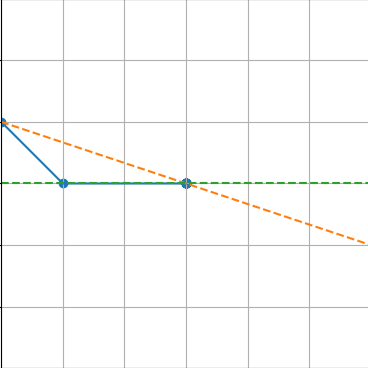
\includegraphics[scale=0.7]{1new.png} 
  \caption{Метод Якоби}
\end{figure}

Ассимптотические прямые возникают из уравнений:
\begin{equation*}
x^{k+1} = b_{12} y^k + c_1
\end{equation*}
\begin{equation*}
y^{k+1} = b_{21} x^k + c_2
\end{equation*}\\


\begin{figure}[h]
  \centering 
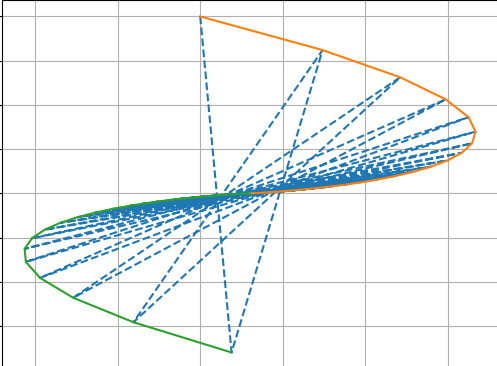
\includegraphics[scale=0.7]{2new.png} 
  \caption{Метод Зейделя}
\end{figure}

\begin{equation*}
x^{k+1} = b_{12} y^k + c_1
\end{equation*}
\begin{equation*}
y^{k+1} = b_{21} x^k + c_2
\end{equation*}\\

где: $b_{12} = - \frac{a_{12}}{a_{11}}$, $c_1 = \frac{b_1}{a_{11}}$, $b_{21} = - \frac{a_{21}}{a_{22}}$, $c_2=\frac{b_2}{a_{22}}$.
\newpage


\begin{figure}[h]
  \centering 
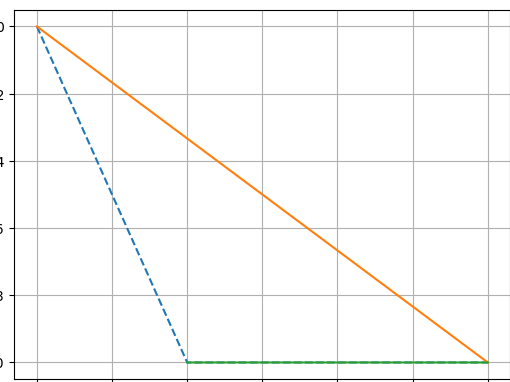
\includegraphics[scale=0.7]{3new.png}
  \caption{Метод релаксации}
\end{figure}
 
 \begin{equation*}
x^{k+1} = \left( 1 - \omega \right) x^k + \omega B_1 x^{k+1} + \omega B_2 x^k + \omega c
\end{equation*}\\




\subsection*{№ 4}

\textbf{При каких условиях сходятся метод простой итерации,
метод Якоби, метод Зейделя и метод релаксации? Какую
матрицу называют положительно определенной?}\\

Вообще говоря, условие $\lVert C \rVert<1$ гарантирует сходимость любых методов. Но если говорить в отдельности для каждого, то:\\
1) \textbf{Метод простой итерации} сходится, если, как мы доказывали выше, $\tau < \frac{2}{\lambda_{\max}}$.\\
2) \textbf{Метод Якоби} сходится если выполняется диагональное преобладание:\\
$|a_{ij}|>\sum_{j \neq i} |a_{ij}|$\\
3) \textbf{Метод релаксации} сходится, если коэффициент $\omega$ находится в промежутке $(0,2)$.\\ А так как, в \textbf{методе Зейделя} $\omega = 1$, то он сходится всегда.\\

Для положительно определённой есть много эквивалентных определний, одно из них:\\
Матрица называется положительно определённой, если соответствующая ей квадратичная форма положительна для любого вектора. Другими словами: $(Ax, x)>0 $ для $\forall x \neq 0$.



\subsection*{№ 5}

\textbf{Выпишите матрицу $C$ для методов Зейделя и релаксации.}\\

Метод релаксации представляется в виде:\\
\begin{equation}
    (D+\omega L) \frac{x^{k+1} - x^{k}}{\omega} + Ax^k = b
\end{equation}
\\
\begin{equation}
    (D+\omega L) x^{k+1} + (-D-\omega L + \omega A) x^k = \omega b
\end{equation}
    

\begin{equation}
    x^{k+1} = (D+\omega L)^{-1} \cdot (-\omega A + D + \omega L)x^k + (D+\omega L)^{-1}\omega b
\end{equation}
\\ Далее используя определения матриц $L-A = -D -U$, получаем матрицу $C$ как коэффициент перед $x^k$ для метода релаксации: 
\begin{equation}
    C=(D+\omega L)^{-1} \cdot ((1-\omega)D-\omega U)
\end{equation}
\\И также для метода Зейделя ($\omega = 1$): 
\begin{equation}
    C=(D+ L)^{-1} U
\end{equation}



\subsection*{№ 6}

\textbf{Почему в общем случае для остановки итерационного процесса нельзя использовать критерий $\vert \vert x^k - x^{k-1} \vert \vert < \epsilon$?\\}

Если метод сходится довольно медленно, то норма разницы векторов станет довольно маленькой. В таком случае алгоритм совершит ошибку второго рода, и остановится слишком рано. \\


\subsection*{№ 7}
\textbf{Какие еще критерии окончания итерационного процесса Вы можете предложить? \\}

\begin{equation*}
    \vert Ax^k - b \vert \leq \epsilon
\end{equation*}
\begin{equation*}
\vert \vert x^{k+1} - x^{k} \vert \vert \leq \frac{1 - \vert \vert C \vert \vert }{\vert \vert C \vert \vert} \cdot \epsilon
\end{equation*}
\begin{equation*}
\vert \vert x_{k+1} - x_{k} \vert \vert \leq \epsilon \vert \vert x_k \vert \vert + \epsilon_{0}
\end{equation*}






\end{document}
